\chapter{A prototype of a machine learning workflow to classify land use} \label{ch:ml_workflow}

As was previously mentioned in section~\ref{sec:teranet_challenges_solution}, one of the major features missing from the available version of Teranet's dataset is the information about the type of property being transacted, which introduces a major limitation on how Teranet's data can be used.
As was described in chapter~\ref{ch:data_preparation}, parcel-level land use information from DMTI and the Department of Geography has been spatially joined to Teranet records, but these sources of land use information also have their limitations:

\begin{itemize}
    \item DMTI's land use data does not offer any split between subcategories of residential properties and only covers the period of 2001--2014
    \item land use from the Department of Geography is a lot more detailed and accurate, but has been collected at a single point in time over the summer of 2012 and 2013
    \item neither of the available land use sources covers the full span of the Longitudinal Housing Market Research conducted by UTTRI (1986-2016)
\end{itemize}

\begin{figure}[hbt!]
    \centering
    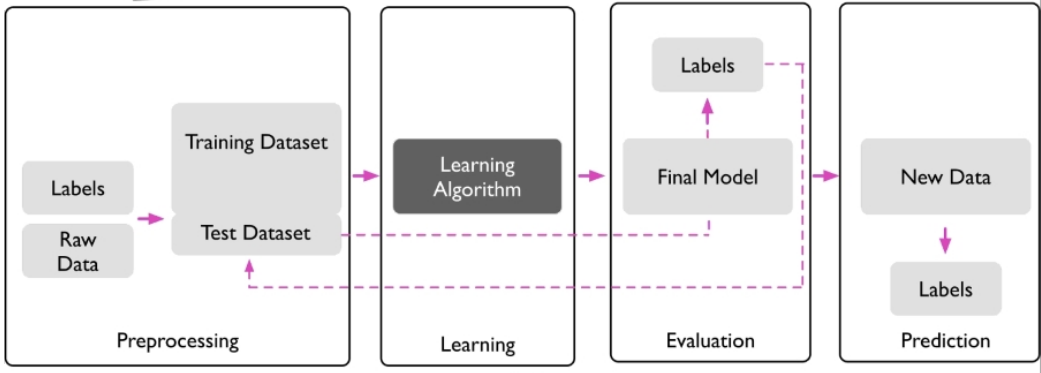
\includegraphics[width=0.98\linewidth,trim=0 0 0 0,clip]{typical_ml_workflow.png}
    \caption{A typical workflow for using machine learning in predictive modeling, as summarized by Raschka and Mirjalili\cite{RaschkaMirjalili2017}.}
    \label{fig:typical_ml_workflow}
\end{figure}

To address this issue, detailed land use from the Department of Geography can be used as labelled data to train a machine learning model capable of recognizing certain property types that have characteristically different behavior on the housing market;
i.e., be able to differentiate a detached house from a condo through such features as high / low volume of transactions, ratio of price to median price for that year, etc.
Chapter~\ref{ch:data_preparation} described the production of the dataset that combines the new features engineered from Teranet data with spatially-joined variables from Census and TTS\@.
In this chapter, this dataset is used to investigate the opportunity to implement a classification algorithm to determine the parcel land use at Teranet transaction level (recognizing changes of land use with time) based on the housing market dynamics.
This way, a machine learning algorithm could provide a scalable solution to automate a labour-intensive task of collecting parcel-level detailed land use and expand the temporal span for which the land use data collected from the Department of Geography can be used with accuracy.

Figure~\ref{fig:typical_ml_workflow} presents a typical workflow for using machine learning in predictive modeling, as summarized by Raschka and Mirjalili\cite{RaschkaMirjalili2017}.

\section{Selecting and encoding the target variable} \label{sec:select_encode_target}

As was expected, different property types have characteristically different behaviour on the housing market.
Figure~\ref{fig:xy_total_sales_dist_by_lu} shows the distributions of total count of Teranet records per 'xy' coordinate pair by the top 10 land use categories.

\begin{figure}[hbt!]
    \centering
    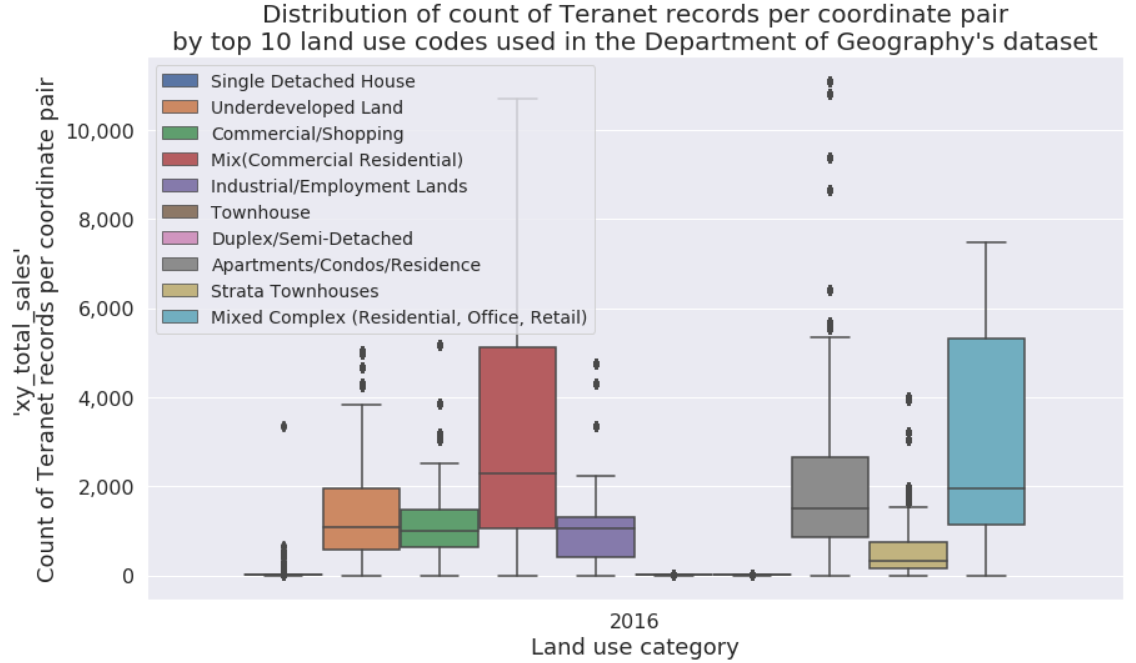
\includegraphics[width=0.98\linewidth,trim=0 0 0 0,clip]{xy_total_sales_dist_by_lu.png}
    \caption{Distributions of total count of Teranet records per 'xy' coordinate pair by top 10 land use categories.
    It can be seen that detached houses, duplexes, and townhouses ("collapsed" boxplots) have much lower number of records per 'xy'.
    It can also be seen that there are some outliers present on the category of detached houses (first boxplot from the left), which most likely represent mislabelled records, as it is very unlikely that a detached house can have almost 4'000 sales.}
    \label{fig:xy_total_sales_dist_by_lu}
\end{figure}

The target variable used for the purposes of investigating the possibility of land use classification was constructed by reducing the land use codes used in the Department of Geography's dataset to 4 major categories;
these categories were derived from the land use codes that have the highest counts of Teranet records.
The four classes that were manually selected as a reduced representation of the major property types have been chosen to have a comparable number of records between classes and a similar distribution of price and count of sales per 'xy' between the land use categories that were grouped together to form a single class.
Figure~\ref{fig:class_2_price_dist} shows an example of such grouping: in class 2, Duplex/Semi-Detached properties are grouped together with Townhouses.

\begin{figure}[ht]
    \centering
    \begin{subfigure}{\linewidth}
        \centering
        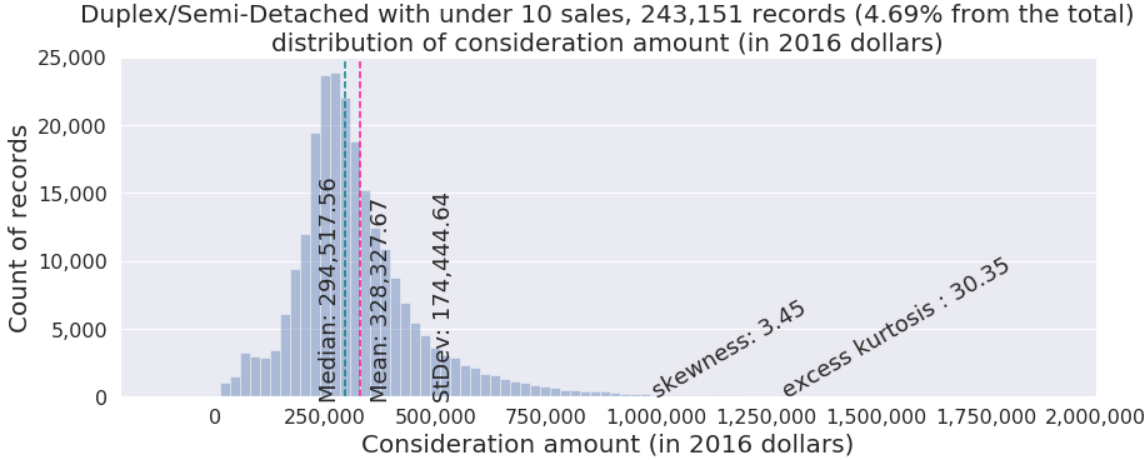
\includegraphics[width=.98\linewidth]{duplex_price_dist.png}
        \label{fig:duplex_price_dist}
        \caption{Duplex/Semi-Detached}
    \end{subfigure}

    \begin{subfigure}{\linewidth}
        \centering
        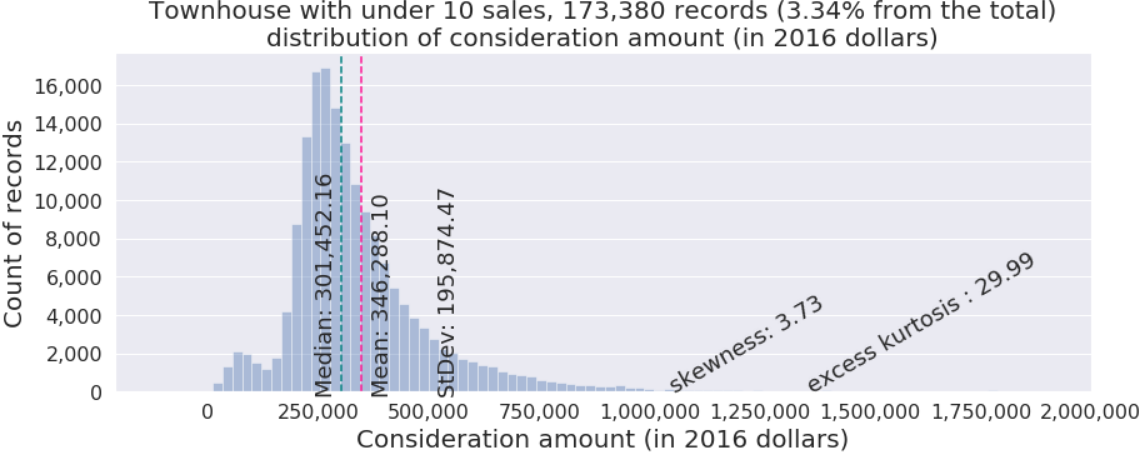
\includegraphics[width=.98\linewidth]{townhouse_price_dist.png}
        \label{fig:townhouse_price_dist}
        \caption{Townhouse}
    \end{subfigure}
    \caption{Distribution of price (in 2016 dollars) for two property types grouped together under Class 2: Townhouses and Duplex/Semi-Detached.
    Both categories have similar distributions of price and records per 'xy' and thus are grouped together to represent a single class "duplex\_townhouse".}
    \label{fig:class_2_price_dist}
\end{figure}

The four target classes that were introduced are:

\begin{itemize}
    \item Class 0: "condo", including Apartments/Condos/Residence and Strata Townhouses
    \item Class 1: "detached", including Single Detached Houses
    \item Class 2: "duplex\_townhouse", including Duplex/Semi-Detached and Townhouses
    \item Class 3: "other", including Commercial/Shopping, Mix (Commercial Residential), Industrial/Employment Lands, and everything else
\end{itemize}

The selection was performed with an aim to separate types of properties that would have characteristically different behaviour on the housing market (i.e., detached houses would have a much smaller frequency of transaction when compared to condos and a higher median price when compared to duplexes).
Distributions of price (in 2016 dollars) and count of records per 'xy' coordinate pair were used to define classes.
Figure~\ref{fig:class_2_price_dist} presents an example of price distributions for Townhouses and Duplex/Semi-Detached.
Similar analysis has been performed to group other categories together into 4 major classes.

Classification algorithms, a subcategory of algorithms for supervised learning, predict the discrete unordered categorical class labels of new instances based on past observations.
A trained algorithm is capable of using a set of rules that were learned from past observations to distinguish new instances between the possible classes.
Once the classes have been determined and assigned, the target variable must be encoded, as it is considered good practice to provide class labels as integer arrays to avoid technical glitches and improve computational efficiency.
Class labels are not ordinal and classification estimators in scikit-learn\cite{scikit-learn} machine learning library in Python treat class labels as categorical data that does not imply any order.
'LabelEncoder' from scikit-learn was used to encode the class labels as integers.

\section{Dimensionality reduction} \label{sec:dimensionality_reduction}

The quality of the data plays a critical part in the success of the application of a machine learning algorithm, and one of the important aspects of data quality is the dimensionality of the input space.
The input space may contain features that are either redundant or irrelevant;
highly correlated features also introduce multicollinearity and can make the model unstable, or too sensitive to small changes in the input data.
In machine learning, statistics, and information theory, dimensionality reduction is the process of reducing the number of random variables under consideration.
There is a number of reasons for reducing dimensionality of a dataset:

\begin{enumerate}
    \item reducing the number of features improves computational efficiency and reduces training times
    \item in case of a low signal-to-noise ratio in the dataset, dimensionality reduction can improve the predictive performance of an algorithm\cite{RaschkaMirjalili2017}
    \item simpler models are easier to interpret\cite{James2013}
    \item excessive complexity of the model could cause overfitting\cite{RaschkaMirjalili2017}
    \item the curse of dimensionality\cite{Bellman1954} (in the context of machine learning, the curse of dimensionality describes the phenomena where the feature space becomes too sparse for the size of the training dataset)\cite{RaschkaMirjalili2017}
\end{enumerate}

There is a number of approaches that could be utilized to reduce the dimensionality of the feature space.
There are two main categories of dimensionality reduction techniques:
\begin{itemize}
    \item feature selection, also referred to as Feature Subset Selection, or (FSS), where a subset of the original features is selected
    \item feature extraction, where a new feature subspace is constructed from information derived from the original feature set
\end{itemize}

A feature selection algorithm presents a practical approach to feature selection at scale;
such algorithms combine a search strategy for proposing new feature subsets with an objective function to evaluate these subsets.
Exhaustive evaluation of all possible feature subsets is computationally unfeasible even for a moderate number of features.
For example, if we are given a feature set with $m = 64$ features and want to reduce it to $n = 19$, an exhaustive evaluation would involve over $10^{15}$ possible feature sets:

\begin{equation}
    _{m}C_n = _{64}C_{19} = \binom{64} {19} = \frac{64!} {19!(64 - 19)!} = 8,719,878,125,622,720
\end{equation}

Therefore, it is more practical to utilize an FSS algorithm that uses some other search strategy to explore the space of all possible combinations of features.
The second element of a feature selection algorithm is the objective function, which plays the role of a feedback signal used by the search strategy to choose between candidate subset.
Objective functions are divided into three major groups:

\begin{itemize}
    \item filters
    \begin{itemize}
        \item evaluate candidate feature subsets by their information content (e.g., inter/intra class distance, mutual information, etc.)
        \item advantages: have faster execution since there generally is no iterative computation;
        have good generality since they evaluate the intrinsic properties of the data.
        \item disadvantages: tend to select large feature subsets due to monotonic objective functions
    \end{itemize}
    \item wrappers
    \begin{itemize}
        \item use a classifier to evaluate subsets by their predictive accuracy on test data
        \item advantages: have better accuracy since they select subsets based on specific interactions between the classifier and the dataset
        \item disadvantages: slower to execute since a classifier needs to be re-trained multiple times;
        selected feature subset will be specific to the classifier that was used to evaluate the candidate subsets.
    \end{itemize}
    \item embedded methods
    \begin{itemize}
        \item feature selection is performed as a part of model construction process (i.e., LASSO method for constructing a linear model with L1 regularization)\cite{Scikit-learndevelopers2019}
        \item
    \end{itemize}
\end{itemize}
An example of a feature selection algorithm is the Sequential Backward Selection algorithm

To gain a better understanding of the data, univariate feature selection techniques can be used;
these techniques examine each feature individually to determine the strength of the relationship of a feature with the target variable.
Univariate feature selection methods could be useful for better understanding of the data, but not necessarily for improving the generalization of the learning algorithm.

One of the simplest methods to analyze the relationship between individual features and the target classes is the Pearson correlation coefficient, measuring bivariate correlation.
The values of the coefficient lie in the interval $[-1; 1]$, with $-1/+1$ meaning perfect negative/positive correlation respectively, and 0 meaning no linear correlation between the two variables.
However, it is important to remember that Pearson correlation coefficient is only sensitive to a linear relationship between the variables and can be close to 0 even if a strong non-linear relationship is present.
Figure~\ref{fig:sbs9f_corr} presents an example of a plot displaying 9 selected features (selection process is described below) and their Pearson correlation coefficients with each target class (target classes have been encoded one-hot for this purpose).
Similar analysis was performed on the full list of 54 features as a first step in assessing their importance.

\begin{figure}[hbt!]
    \centering
    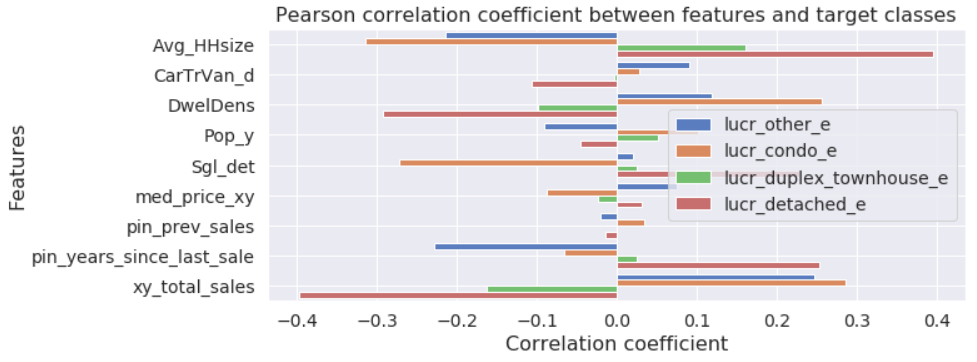
\includegraphics[width=0.98\linewidth,trim=0 0 0 0,clip]{sbs9f_corr.png}
    \caption{9 most important features determined using Sequential Backward Selection (SBS) algorithm and their Pearson correlation coefficients for each target class.
    Target classes have been encoded one-hot for the purposes of this plot.}
    \label{fig:sbs9f_corr}
\end{figure}

Interpreting the relationships between the two variables based solely on correlation value can be highly misleading, as illustrated by Anscombe's quartet\cite{Anscombe1973}, which highlights the importance of visualization.
Pair-wise scatter plots have been produced for all variables to analyze their distributions by target classes, figure~\ref{fig:pairplot_sample} presents a section of such pairplot.

\begin{figure}[hbt!]
    \centering
    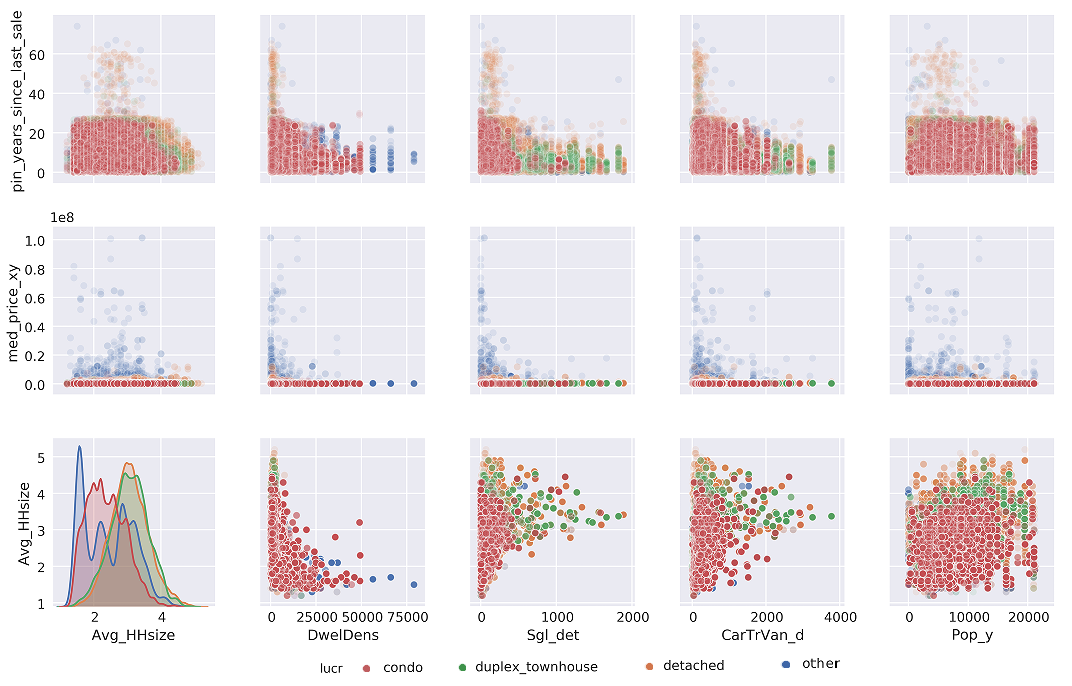
\includegraphics[width=0.98\linewidth,trim=0 0 0 0,clip]{pairplot_sample.png}
    \caption{A section of a pairplot with pair-wise scatter plots of input variables coloured by target classes.}
    \label{fig:pairplot_sample}
\end{figure}

Another possible approach to reduce the complexity of a model is to use L1 regularization to penalize large individual weights.
L1 regularization introduces a penalty term to the cost function which is taken as the norm of the weight vector defined as:

\begin{equation} \label{eq:l1_regularization}
    L1:~\norm{\vect{w}}_1 = \sum \limits_{j=1}^m \abs{w_j}
\end{equation}

L1 regularization is similar to L2 regularization, which is defined as:

\begin{equation} \label{eq:l2_regularization}
    L2:~\norm{\vect{w}}_2^2 = \sum \limits_{j=1}^m w_j^2
\end{equation}
where $m$ is the number of features.

However, since in the case of L1 regularization, the sum of squares of weights is replaced with the sum of the absolute values of weights, L1 regularization usually yields sparse feature vectors, since most feature weights will be zero\cite{RaschkaMirjalili2017,Scikit-learndevelopers2019}.
Sparsity of feature vectors can help us get rid of irrelevant features in a high-dimensional dataset;
in this context, L1 regularization can be understood as a technique for feature selection\cite{RaschkaMirjalili2017}.
Figure~\ref{fig:lr_l1_sbs9f_coef} presents the plot of model coefficients for each class that were obtained from a Logistic Regression model with L1 regularization.

\begin{figure}[hbt!]
    \centering
    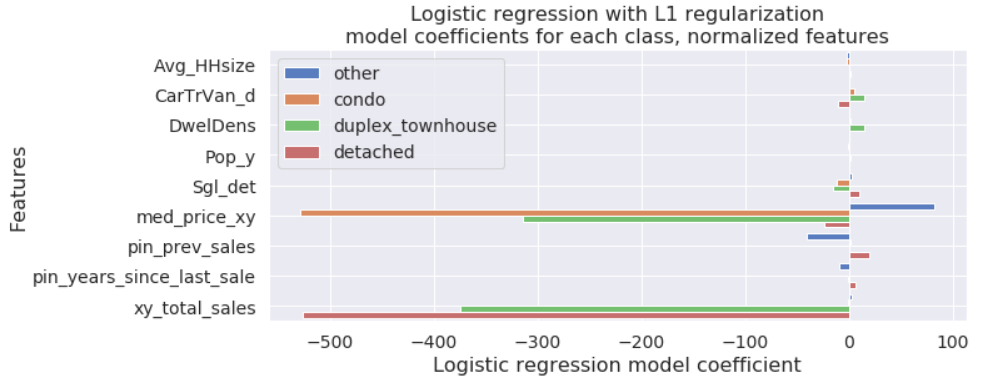
\includegraphics[width=0.98\linewidth,trim=0 0 0 0,clip]{lr_l1_sbs9f_coef.png}
    \caption{Logistic regression with L1 regularization, model coefficients.}
    \label{fig:lr_l1_sbs9f_coef}
\end{figure}



\section{Training, testing and validating the model} \label{sec:train_test_validate_model}

\textit{To determine whether our machine learning algorithm not only performs well on the training set but also generalizes well to new data, we also want to randomly divide the dataset into a separate training and test set. We use the training set to train and optimize our machine learning model, while we keep the test set until the very end to evaluate the final model.}

\textit{comparing predictions to true labels in the test set can be understood as the unbiased performance evaluation of our model}

\textit{For example, each classification algorithm has its inherent biases, and no single classification model enjoys superiority if we don't make any assumptions about the task. In practice, it is therefore essential to compare at least a handful of different algorithms in order to train and select the best performing model. But before we can compare different models, we first have to decide upon a metric to measure performance. One commonly used metric is classification accuracy, which is defined as the proportion of correctly classified instances.}

\textit{After we have selected a model that has been fitted on the training dataset, we can use the test dataset to estimate how well it performs on this unseen data to estimate the generalization error. If we are satisfied with its performance, we can now use this model to predict new, future data. It is important to note that the parameters for the previously mentioned procedures, such as feature scaling and dimensionality reduction, are solely obtained from the training dataset, and the same parameters are later reapplied to transform the test dataset, as well as any new data samples—the performance measured on the test data may be overly optimistic otherwise.}

\textit{randomly partition this dataset into separate test and training datasets is to use the train_test_split function from scikit-learn's model_selection submodule:}

\textit{In this context, stratification means that the train\_test\_split method returns training and test subsets that have the same proportions of class labels as the input dataset.}

\section{Feature scaling} \label{sec:feature_scaling}

\textit{Raw data rarely comes in the form and shape that is necessary for the optimal performance of a learning algorithm. Thus, the preprocessing of the data is one of the most crucial steps in any machine learning application. Many machine learning algorithms also require that the selected features are on the same scale for optimal performance, which is often achieved by transforming the features in the range [0, 1] or a standard normal distribution with zero mean and unit variance, as we will see in later chapters.}

\textit{Decision trees and random forests are two of the very few machine learning algorithms where we don't need to worry about feature scaling. Those algorithms are scale invariant.}

\textit{there are two common approaches to bring different features onto the same scale: normalization and standardization.}

\textit{Most often, normalization refers to the rescaling of the features to a range of [0, 1], which is a special case of min-max scaling. To normalize our data, we can simply apply the min-max scaling to each feature column, where the new value x_{norm}^{(i)} of a sample x^{(i)} can be calculated as follows:}

\begin{equation} \label{eq:normalization}
    x_{norm}^{(i)} = \frac{x^{(i)} - x_{min}} {x_{max} - x_{min}}
\end{equation}

Here, $x^{(i)}$ is a particular sample, $x_{\min}$ is the smallest value in a feature column, and  the largest value.

The min-max scaling procedure is implemented in scikit-learn via MinMaxScaler.

\textit{Although normalization via min-max scaling is a commonly used technique that is useful when we need values in a bounded interval, standardization can be more practical for many machine learning algorithms, especially for optimization algorithms such as gradient descent. The reason is that many linear models, such as the logistic regression and SVM that we remember from Chapter 3, A Tour of Machine Learning Classifiers Using scikit-learn, initialize the weights to 0 or small random values close to 0. Using standardization, we center the feature columns at mean 0 with standard deviation 1 so that the feature columns have the same parameters as a standard normal distribution (zero mean and unit variance), which makes it easier to learn the weights. Furthermore, standardization maintains useful information about outliers and makes the algorithm less sensitive to them in contrast to min-max scaling, which scales the data to a limited range of values.}

\textit{standardization, which gives our data the property of a standard normal distribution, which helps gradient descent learning to converge more quickly. Standardization shifts the mean of each feature so that it is centered at zero and each feature has a standard deviation of 1. For instance, to standardize the jth feature, we can simply subtract the sample mean  from every training sample and divide it by its standard deviation :. One of the reasons why standardization helps with gradient descent learning is that the optimizer has to go through fewer steps to find a good or optimal solution (the global cost minimum)}

The procedure for standardization can be expressed by the following equation:

\begin{equation} \label{eq:standardization}
    \vect{x}^{(i)}_{std} = \frac{\vect{x}^{(i)} - \mu_x}{\sigma_x}
\end{equation}

\textit{Here,  is a vector consisting of the jth feature values of all training samples n, and this standardization technique is applied to each feature j in our dataset.}

\textit{we fit the StandardScaler and MinMaxScaler classes only once—on the training data—and use those parameters to transform the test set or any new data point.}

\section{Classification algorithms and their performance} \label{sec:classification_algorithms_performance}

\textit{Machine learning algorithms can be grouped into parametric and nonparametric models. Using parametric models, we estimate parameters from the training dataset to learn a function that can classify new data points without requiring the original training dataset anymore. Typical examples of parametric models are the perceptron, logistic regression, and the linear SVM. In contrast, nonparametric models can't be characterized by a fixed set of parameters, and the number of parameters grows with the training data. Two examples of non-parametric models that we have seen so far are the decision tree classifier/random forest and the kernel SVM.}

An important point to be summarized from the famous No Free Lunch Theorems (NFL)\cite{Wolpert1996,Wolpert1997} by David H. Wolpert is that no single classifier works best across all possible scenarios, as there is a lack of a priori distinctions between learning algorithms.

\textit{For example, each classification algorithm has its inherent biases, and no single classification model enjoys superiority if we don't make any assumptions about the task. In practice, it is therefore essential to compare at least a handful of different algorithms in order to train and select the best performing model. But before we can compare different models, we first have to decide upon a metric to measure performance. One commonly used metric is classification accuracy, which is defined as the proportion of correctly classified instances.}

\textit{In practice, it is always recommended that you compare the performance of at least a handful of different learning algorithms to select the best model for the particular problem; these may differ in the number of features or samples, the amount of noise in a dataset, and whether the classes are linearly separable or not.}

\textit{Trying to understand how the biological brain works, in order to design AI, Warren McCulloch and Walter Pitts published the first concept of a simplified brain cell, the so-called McCulloch-Pitts (MCP) neuron, in 1943 (A Logical Calculus of the Ideas Immanent in Nervous Activity, W. S. McCulloch and W. Pitts, Bulletin of Mathematical Biophysics, 5(4): 115-133, 1943).}

\textit{Only a few years later, Frank Rosenblatt published the first concept of the perceptron learning rule based on the MCP neuron model (The Perceptron: A Perceiving and Recognizing Automaton, F. Rosenblatt, Cornell Aeronautical Laboratory, 1957). With his perceptron rule, Rosenblatt proposed an algorithm that would automatically learn the optimal weight coefficients that are then multiplied with the input features in order to make the decision of whether a neuron fires or not. In the context of supervised learning and classification, such an algorithm could then be used to predict if a sample belongs to one class or the other.}

\textit{Another simple yet more powerful algorithm for linear and binary classification problems: logistic regression. Note that, in spite of its name, logistic regression is a model for classification, not regression.}

\texiit{Logistic regression is a classification model that is very easy to implement but performs very well on linearly separable classes. It is one of the most widely used algorithms for classification in industry. Similar to the perceptron and Adaline, the logistic regression model in this chapter is also a linear model for binary classification that can be extended to multiclass classification, for example, via the OvR technique.}

\textit{Decision trees can build complex decision boundaries by dividing the feature space into rectangles. Decision tree classifiers are attractive models if we care about interpretability. As the name decision tree suggests, we can think of this model as breaking down our data by making a decision based on asking a series of questions. Based on the features in our training set, the decision tree model learns a series of questions to infer the class labels of the samples. Using the decision algorithm, we start at the tree root and split the data on the feature that results in the largest Information Gain (IG). In an iterative process, we can then repeat this splitting procedure at each child node until the leaves are pure. This means that the samples at each node all belong to the same class. In practice, this can result in a very deep tree with many nodes, which can easily lead to overfitting. Thus, we typically want to prune the tree by setting a limit for the maximal depth of the tree. As we can see, the information gain is simply the difference between the impurity of the parent node and the sum of the child node impurities — the lower the impurity of the child nodes, the larger the information gain. Now, the three impurity measures or splitting criteria that are commonly used in binary decision trees are Gini impurity ($I_G$), entropy ($I_H$), and the classification error ($I_E$).}

\textit{Random forests have gained huge popularity in applications of machine learning during the last decade due to their good classification performance, scalability, and ease of use. Intuitively, a random forest can be considered as an ensemble of decision trees. The idea behind a random forest is to average multiple (deep) decision trees that individually suffer from high variance, to build a more robust model that has a better generalization performance and is less susceptible to overfitting.}

1. Draw a random bootstrap sample of size n (randomly choose n samples from the training set with replacement).

2. Grow a decision tree from the bootstrap sample. At each node:

a. Randomly select d features without replacement.

b. Split the node using the feature that provides the best split according to the objective function, for instance, maximizing the information gain.

3. Repeat the steps 1-2 k times.

4. Aggregate the prediction by each tree to assign the class label by majority vote.

\textit{In most implementations, including the RandomForestClassifier implementation in scikit-learn, the size of the bootstrap sample is chosen to be equal to the number of samples in the original training set, which usually provides a good bias-variance tradeoff. For the number of features d at each split, we want to choose a value that is smaller than the total number of features in the training set. A reasonable default that is used in scikit-learn and other implementations is $d=\sqrt{m}$, where m is the number of features in the training set.}

\textit{Although we are growing a very small random forest from a very small training dataset, we used the n\_jobs parameter for demonstration purposes, which allows us to parallelize the model training using multiple cores of our computer (here two cores).}

\textit{k-nearest neighbor (KNN) classifier is particularly interesting because it is fundamentally different from the learning algorithms that we have discussed so far.  KNN is a typical example of a lazy learner. It is called lazy not because of its apparent simplicity, but because it doesn't learn a discriminative function from the training data, but memorizes the training dataset instead. KNN belongs to a subcategory of nonparametric models that is described as instance-based learning. Models based on instance-based learning are characterized by memorizing the training dataset, and lazy learning is a special case of instance-based learning that is associated with no (zero) cost during the learning process.}

The KNN algorithm itself is fairly straightforward and can be summarized by the following steps:

1. Choose the number of k and a distance metric.

2. Find the k-nearest neighbors of the sample that we want to classify.

3. Assign the class label by majority vote.

\section{Chapter summary} \label{sec:ml_workflow_summary}
asd